\todo{introduction}

\section{Intersection Theory}

Throughout, let's assume $X$ is an ambient $n$-dimensional closed manifold.

\begin{definition}
	Two submanifolds $M,N\subset X$ are said to \defn{intersect tranversally} or to be \defn{transverse} if for all points $p\in M\cap N$ we have $\T_p M\oplus \T_p N = \T_p X$.
\end{definition}

	\begin{figure}[ht]
		\centering
		\import{graphics/temp-diagrams/}{transverse-intersection.pdf_tex}
		\medskip
		\caption{Examples and non-examples of transverse intersections in $\R^3$.}\label{fig:transverse-intersection}
	\end{figure}

	If one of the manifolds isn't smoothly embedded in the ambient space, but rather the image of a smooth map then this definition can be slightly generalized.

\begin{definition}
	If $M\subset X$ is a submanifold and $f : N \to X$ is a smooth map, we say that $f$ is \defn{transverse} to $M$ if for all points $p\in f^{-1}(M)$ we have $df_p(\T_p N)\oplus \T_{f(p)}M = \T_{f(p)}X$.
\end{definition}

\begin{theorem}[Preimage Theorem]
	\todo{todo}
\end{theorem}

\begin{proposition}
	If $M$ and $N$ are transverse, then $M\cap N$ is also a submanifold.
\end{proposition}

While it's easy to come up with examples of manifolds which aren't transverse, there is a mathematical sense in which ``almost all'' submanifolds intersect transversally.

\begin{theorem}
	Let $C^\infty(N,X)$ be the space of all maps from a compact manifold $N$ to some ambient manifold $X$. If we fix a submanifold $M\subset X$, then the subset
	\[
		T_X(N,M) = \{ f : N \to X \mid f\textrm{ is transverse to } M\}\subset C^\infty(N,X)
	\]
	of maps transverse to $M$ is a dense subset of $C^\infty(N,X)$.
\end{theorem}

\begin{proof}
	\todo{todo}
\end{proof}

% \begin{definition}
% 	Suppose we have a property $\mathcal{P}$ of functions between topological spaces.
% 	\begin{enumerate}
% 		\item The property $\mathcal{P}$ is said to be \defn{stable} if for every function $f : X \to Y$ satisfying $\mathcal{P}$ and homotopy $H : X\times[0,1]\to Y$ with $H(x,0) = f(x)$, there exists an $\varepsilon>0$ such that for all $s\in [0,\varepsilon)$, the function $H(x,s)$ also satisfies $\mathcal{P}$.
% 		\item The property $\mathcal{P}$ is said to be \defn{generic} if for every function $f : X \to Y$ \emph{not} satisfying $\mathcal{P}$ and arbitrary $\varepsilon>0$, there is a homotopy $H : X\times [0,\varepsilon] \to Y$ with $H(x,0)=f(x)$ such that the function $H(x,\varepsilon)$ satisfies $\mathcal{P}$.
% 	\end{enumerate}
% 	\todo{target manifold same}
% \end{definition}
%
% In other words, stability implies that the property is resilient to small perturbations in any direction and generality implies that any function which doesn't satisfy the property can be perturbed slightly so that it does satisfy the property. Transversality fits both of these descriptions.
%
% \begin{theorem}
% 	For smooth maps from a compact manifold $N$ to a manifold $X$, transversality with respect to a fixed submanifold $M\subset X$ is a stable and generic property.
% \end{theorem}

	\begin{figure}[ht]
		\centering
		\import{graphics/temp-diagrams/}{perturbing-intersection-transverse.pdf_tex}
		\medskip
		\caption{Perturbing a manifold to get a transverse intersection.}\label{fig:perturbing-intersections-transverse}
	\end{figure}
This means that without much loss of generality, we can assume that all manifolds and smooth maps intersect transversally.

\subsection*{The Oriented Intersection Number}

Whenever we have a manifold $M\subset X$ and a smooth map $f : N \to X$ intersecting transversally, the preimage theorem implies that there is a submanifold $S = f^{-1}(N)\subset M$ of $M$. 
If all manifolds involved are orientable, this preimage $S$ admits a canonical orientation by the following procedure. 

First of all, recall that for any embedded manifold $M\subset X$ there is an exact sequence of vector bundles by quotienting
\begin{equation}\label{eq:oriented-intersection-number-1}
	\begin{tikzcd}
	0 & {\T M} & {\T X} & {\T X/M} & 0
	\arrow[from=1-1, to=1-2]
	\arrow[from=1-2, to=1-3]
	\arrow[from=1-3, to=1-4]
	\arrow[from=1-4, to=1-5]
	\end{tikzcd}
\end{equation}
where $\T X/M$ is the normal bundle of $M\subset X$. Using the orientations of $X$ and $M$, we can use this exact sequence to get an orientation of the normal bundle $\T X/M$. At every point $p\in S$ of the preimage, the differential map $df$ connects the sequence \cref{eq:oriented-intersection-number-1} to the normal bundle sequence for the embedding $S\subset N$.
\begin{equation}\label{eq:oriented-intersection-number-2}
	\begin{tikzcd}
	0 & {\T_pS} & {\T_p N} & {\T_p N/S} & 0 \\
	0 & {\T_{f(p)}M} & {\T_{f(p)}X} & {\T_{f(p)}X/M} & 0
	\arrow[from=1-1, to=1-2]
	\arrow[from=1-2, to=1-3]
	\arrow["{df_p}", from=1-2, to=2-2]
	\arrow[from=1-3, to=1-4]
	\arrow["{df_p}", from=1-3, to=2-3]
	\arrow[from=1-4, to=1-5]
	\arrow["{df_p}", from=1-4, to=2-4]
	\arrow[from=2-1, to=2-2]
	\arrow[from=2-2, to=2-3]
	\arrow[from=2-3, to=2-4]
	\arrow[from=2-4, to=2-5]
	\end{tikzcd}
\end{equation}
In this diagram \cref{eq:oriented-intersection-number-2}, the rightmost vertical map is an isomorphism by the transversality of $f$ and $M$. This means that we can pullback the orientation on $\T_{f(p)} X/M$ to $\T_p N/S$. Since $\T_p N$ is oriented, the usual ``2-out-of-3'' rule applied to the top row of \cref{eq:oriented-intersection-number-2} gives an orientation of $\T_p S$. See \cref{fig:preimage-orientation} for an example of this orienting procedure.

	\begin{figure}[ht]
		\centering
		\import{graphics/temp-diagrams/}{preimage-orientation.pdf_tex}
		\medskip
		\caption{Orienting a preimage (assuming a clockwise orientation on $X$).}\label{fig:preimage-orientation}
	\end{figure}

	When $

\begin{theorem}\label{thm:euler-characteristic-intersection-number}
	If $M$ is a closed $n$-dimensional submanifold of a $2n$-dimensional submanifold $X$ then we have
	\[
		\iota_*[M]\tnsv \iota_*[M] = \chi(\nu)
	\]
	where $\nu$ is a normal bundle of $M$ in $X$ and $\chi(\nu)$ is its Euler number.
\end{theorem}
\begin{proof}
\end{proof}

\begin{corollary}
	The Euler number $\chi(\xi)$ of an oriented real vector bundle $\xi : E \to B$ over a compact oriented manifold can be expressed as the intersection number
	\[
		z_*[B]\tnsv z_*[B] = \chi(\xi)
	\]
	where $z : B \to E$ is the zero section.
\end{corollary}

\subsection*{Homology Classes and Submanifolds}

Let $f : N\subset X$ be a smooth map from a compact oriented $p$-dimensional manifold $N$ to $X$. The data of an orientation on a closed manifold gives a fundamental class $[N]\in \H_p(N)$ which can be pushed forward along the map $f : N \hookrightarrow X$ to give us a homology class $f_* [N]\in \H_p(X)$. This is the homology class associated to a smooth map $N\to X$.
This correspondence behaves nicely with respect to perturbations, and thus as we will later see, with transversality.
Suppose $H : N\times [0,1] \to X$ is a homotopy with $H(x,0)=f(x)$ which perturbs the map $f$. For any $\varepsilon>0$, the map $f_\varepsilon : N \to X$ given by $f_\varepsilon(x)=H(x,\varepsilon)$ is homotopic to $f$ and hence induces the same map on homology $\H_p(N)\to \H_p(X)$. The homology class associated to a map $f : N \to X$ thus solely depends on the homotopy type of $f$ so we get a map
\[
	\lkxfunc{}{[N,X]}{\H_p(X).}
\]
Letting $N=S^p$, we can see that this is a generalization of the Hurewicz homomorphism which links homotopy groups to homology groups via a map $\pi_p(X) \to \H_p(X)$.
As with the Hurewicz homomorphism, this correspondence is generally not surjective or injective. If a space is $k$-connected for $k\geq 1$ then we have a Hurewicz isomorphism $\pi_{k+1}(X) \to \H_{k+1}(X)$ which means that every homology cycle in $\H_{k+1}(X)$ can at least be represented by a smooth map of a sphere $S^{k+1}$ into $X$. This smooth map might have ``double-points'', i.e. when multiple points of the sphere map to the same point in the image and prevent the smooth map from being an embedding.

\begin{example}
	In the punctured plane $X=\R^2\setminus \{0\}$ with homology $\H_1(X)\cong \Z$, the only homology cycles which can be represented by embedded submanifolds are $0,\pm 1$, by a circle not containing the origin and circles of both orientations surrounding the origin respectively. A smooth map representing a cycle of higher degree would necessarily have a double-point, for instance see \cref{fig:double-point}.
\end{example}

	\begin{figure}[ht]
		\centering
		\import{graphics/temp-diagrams/}{double-point.pdf_tex}
		\caption{A double-point in a smooth map representing $\pm 2\in \H_1(\R^2\setminus\{0\})$.}\label{fig:double-point}
	\end{figure}

\begin{remark}
	In some special cases, homology classes can always be represented by embedded submanifolds. For instance, if $X$ is a $4$-manifold, there are isomorphisms
	\[
		\H^2(X; \Z) \cong [X, K(\Z,2)] \cong [X, \CP^\infty] \cong [X,\CP^2],
	\]
	where the first is the representability of singular cohomology by the Eilenberg-Maclane spectrum, the second identifies $\CP^\infty$ as a $K(\Z,2)$ space, and the third uses the cellular approximation theorem. Any cohomology cycle $\omega\in \H^2(X)$ can be represented by a smooth function $f : X \to \CP^2$. If we choose this function to be transverse to $\CP^1\subset \CP^2$, then $f^{-1}(\CP^1)$ is an embedded $2$-dimensional submanifold of $X$ which corresponds to a Poincar\'e dual class to $\omega$. When $X$ is a compact manifold, Poincar\'e duality tells us that all $2$-dimensional homology cycles can be represented by embedded submanifolds in this way.
\end{remark}

By Poincar\'e-Lefschetz duality for compact manifolds with boundary, there is an isomorphism
\[
	\lkxfunc{}{\H^{n-p}(X,\partial X)}{\H_p(X)}{\omega}{\omega\frown [X,\partial X]}
\]
given an orientation class $[X,\partial X]\in \H_n(X, \partial X)$. Under this duality, there is an elegant geometric interpretation of the cup product on cohomology cycles as the oriented intersection number for submanifolds representing the dual homology cycles (when such a representation is possible).

\[\begin{tikzcd}
		{\H_p(X)\otimes \H_q(X)} & {\H_{n-p-q}(X)} \\
		{\H^{n-p}(X, \partial X)\otimes \H^{n-q}(X,\partial X)} & {\H^{2n-p-q}(X,\partial X)}
		\arrow["\tnsv", from=1-1, to=1-2]
		\arrow["{\cong_\textrm{PD}}", tail reversed, from=1-1, to=2-1]
		\arrow["{\cong_{\textrm{PD}}}", tail reversed, from=1-2, to=2-2]
		\arrow["\smile", from=2-1, to=2-2]
	\end{tikzcd}\]

\begin{theorem}
	Suppose $M,N\subset X$ are transverse oriented submanifolds. Then we have
	\[\iota_*[M]\tnsv \iota_*[N] = \sum_{p\in M\cap N} \sgn(p).\]
\end{theorem}
\begin{proof}
\end{proof}

\begin{definition}
	Let $X$ be an oriented $2m$-dimensional manifold, possibly with boundary. The \defn{intersection form} on middle dimensional homology is the bilinear form
	\[
		\lkxfunc{Q_X}{\H_m(X)_{\mathrm{free}}\otimes \H_m(X)_{\mathrm{free}}}{\Z}{\alpha\otimes \beta}{\alpha\tnsv \beta}
	\]
	where we identify $\H_0(X)\cong \Z$ and $\H_m(X)_{\mathrm{free}}$ denotes the free component of $\H_m(X)$ -- i.e. the quotient by torsion elements.
\end{definition}

\subsection*{Connected Sum}

\begin{figure}[ht]
	\centering
	\import{graphics/temp-diagrams/}{connected-sum.pdf_tex}
	\caption{Construction of the connected sum.}\label{fig:connected-sum}
\end{figure}

\subsection*{Properties of the Intersection Form}

\begin{proposition}\label{prop:symmetry-of-intersection-form}
	If $m$ is even, then $Q_X$ is symmetric and if $m$ is odd, then $Q_X$ is skew-symmetric.
\end{proposition}
\begin{proof}
	\todo{todo}
\end{proof}

\begin{proposition}\label{prop:connected-sum-intersection-form}
	If $X$ and $Y$ are $2m$-dimensional manifolds, then we have
	\[Q_{X\+Y} = Q_X\oplus Q_Y\]
\end{proposition}
\begin{proof}
	\todo{todo}
\end{proof}

\subsection*{Highly-Connected Manifolds}

The simplest class of manifolds for which the intersection form is an interesting invariant are known as highly-connected manifolds. Highly-connected manifolds contain the minimal amount of (co)homological data for which to define an intersection form, and this makes them an attractive target for classification and construction.

\begin{definition}
	A compact $2m$-dimensional manifold $X$ is said to be \defn{highly-connected} if it is $(m-1)$-connected. Consequently, $X$ has non-trivial (co)homology only in the middle dimension $\H_m(X)$ and in the usual extremal dimensions $\H_0(X)$ and $\H_{2m}(X)$.
\end{definition}

\begin{remark}
	In fact, it was the attempted classification of highly-connected manifolds in dimension $8$ which led to the first discovery of an exotic sphere by Milnor in 1956, see \cite{milnor2000exotic} for a historical account of the discvery by the man himself.
\end{remark}

\section{Plumbing}

Suppose we wanted to construct a $2m$-dimensional manifold with a given intersection form -- specified by a bilinear form $Q$ on the unit lattice $\Z^\ell$ with basis vectors $e_1,\ldots, e_\ell$. Let's call this hypothetical construction $P(Q)$.

The simplest possible case is when the lattice is $1$-dimensional, with intersection form
\[
	Q = \begin{pmatrix} Q_{11}\end{pmatrix}
\]
determined by the single integer $Q_{11}=Q(e_1,e_1)\in \Z$.
The resulting $2m$-manifold $P(Q)$ should have middle dimensional homology $\H_m(P(Q))$ free of rank $1$, generated by a cycle $\alpha$ which has self-intersection number $\alpha\tnsv \alpha = Q_{11}$. To construct such a manifold, let's start with a $m$-dimensional sphere $S^m$. This will be the submanifold representing the generating cycle $\alpha\in \H_m(X)$. To get a $2m$-dimensional manifold, we ``thicken'' the sphere by choosing a disk bundle $\xi : E \to S^m$ with Euler number $Q_{11}$ (if such a bundle exists). Note that this is equivalent to choosing a vector bundle, since and we can move freely between vector and disk bundles by an associated bundle construction. We can now define $P(Q)$ as the total space $E$ of the disk bundle. This will be the base case for plumbing constructions.
\begin{figure}[ht]
	\centering
	\import{graphics/temp-diagrams/}{thickening-sphere.pdf_tex}
	\caption{Two different ``thickenings'' of $S^1$ by $D^1$ bundles.}\label{fig:thickening-sphere}
\end{figure}

Although plumbing non-orientable bundles is certainly possible and interesting in its own right, to keep the resulting manifolds orientable we'll require orientable bundles $\xi$ (this rules out the M\"obius bundle thickening in \cref{fig:thickening-sphere}). With this requirement, $P(Q)$ gets a manifold orientation from the orientation of the bundle.
Since disks are contractible, there is a deformation retraction $P(Q)\simeq S^m$, and this implies that the middle dimensional homology $\H_m(X)$ is generated by $\iota_*[S^m]$. By \cref{thm:euler-characteristic-intersection-number} the self intersection number of $\iota_*[S^m]$ is exactly the Euler number $\chi(\xi)$ which we set to be $Q_{11}$ by our choice of bundle $\xi$.

Vector bundles with a given Euler number don't always exist over an $m$-sphere. For instance, if $m$ is odd, then the Euler number of any bundle over $S^m$ is zero and so $Q_{11}$ must be zero in this case. This isn't a failure of the construction but rather reflects that $Q$ is skew-symmetric when $m$ is odd and so must have zeroes along the diagonal. When $m$ is even however, there are plenty of bundles which have a non-zero Euler number. For instance, the tangent bundle $\T S^m$ has Euler number $2$. This lets us construct a $4k$-manifold with boundary that has intersection form $Q = (2)$.

\subsection*{Vector Bundles Over Spheres}

This is a good time for a brief interlude on vector bundles over spheres.
Vector bundles over a sphere can be classified by the clutching construction. Suppose $\xi : E \to S^m$ is a vector bundle. We can decompose the sphere $S^m$ into hemispheres $S^m=D_+^m\cup D_-^m$, and these disks intersect at the equator $D_+^m\cap D_-^m=S^{m-1}\subset S^m$ -- a sphere one dimension lower. The bundle $\xi$ can be trivialized on the hemispheres since they are contractible, and we denote these trivializations
\[
	\lkxfunc{\varphi_+}{E|_{D^m_+}}{D^m_+\times \R^m}
	\quad\textrm{and}\quad
	\lkxfunc{\varphi_-}{E|_{D^m_-}}{D_-^m \times \R^m.}\]
The trivializations must come with transition functions on their intersection (we might have to expand the intersection a bit so that it is open). The transition function is a diffeomorphism $\psi$ in the commutative diagram
\[\begin{tikzcd}
		{S^{m-1}\times \R^m} && {S^{m-1}\times \R^m} \\
		& {E|_{S^{m-1}}}
		\arrow["\psi", from=1-1, to=1-3]
		\arrow["{\varphi_+|_{S^{m-1}}}", from=2-2, to=1-1]
		\arrow["{\varphi_-|_{S^{m-1}}}"', from=2-2, to=1-3]
	\end{tikzcd}\]
which is constant on the first factor, and linear in the second factor. For each point $p\in S^{m-1}$, the diffeomorphism $\psi$ thus gives a linear function $\tau_p : \R^m \to \R^m$. These linear maps are the ``change of coordinate'' transformations between the fibers on the boundaries of $D_+^m$ and $D_-^m$ (see \cref{fig:clutching-construction}).
\begin{figure}[ht]
	\centering
	\import{graphics/temp-diagrams/}{clutching-construction.pdf_tex}
	\caption{Getting a map $\tau : S^{m-1}\to \GL_m$ from a vector bundle over $S^{m}$.}\label{fig:clutching-construction}
\end{figure}

Altogether, this family of linear transformations is indexed by the equator $S^{m-1}$, and this gives us a smooth map $\tau : S^{m-1}\to \GL_m$. It follows that the homotopy type of $\tau$ is only dependent on the isomorphism type of the bundle $\xi$ since any vector bundle isomorphism can be shown to induce a homotopy of smooth maps. In order words, we have a map
\[
	\lkxfunc{}{\op{Vect}_m(S^m)}{\pi_{m-1}(\GL_m).}
\]
sending a vector bundle $\xi$ to the its associated homotopy class $\tau\in \pi_{m-1}(\GL_m)$.

The construction works in the opposite direction as well. Whenever we have a homotopy class $\tau\in \pi_{m-1}(\GL_m)$, we can form a bundle $\xi_\tau : E_\tau \to S^{m}$ by letting
\[
	E_\tau = (D_+^m\times D^m)\cup_T (D_-^{m}\times D^m),
\]
where $T(x,y)=(x,\tau(x)y)$ is the glueing map.

\todo{write this}

A similar argument holds when we restrict to oriented bundles, i.e. vector bundles with structure group $\SO_m$.

\begin{theorem}
	The clutching construction gives bijections
	\[
		\begin{aligned}
			\lkxfunc{}{\pi_{m-1}(\O_m)}{\op{Vect}_m(S^m)} \\
			\lkxfunc{}{\pi_{m-1}(\SO_m)}{\op{Vect}_m^+(S^m)}
		\end{aligned}
	\]
	between homotopy groups of the orthogonal groups and isomorphism classes of vector bundles.
\end{theorem}
\begin{proof}
	\todo{prove}
\end{proof}

Under this correspondence the Euler number of a vector bundle can be considered as a group homomorphism
\[
	\lkxfunc{e}{\pi_{m-1}(\SO_m)}{\Z}{\tau}{e(\xi_\tau)}
\]
\begin{theorem}\label{thm:euler-number-of-vector-bundle-over-sphere}
	Let $p : \SO_{2m} \to \SO_{2m}/\SO_{2m-1}= S^{2m-1}$ be the projection map of the special orthogonal group to the sphere. Then the following diagram commutes,
\[\begin{tikzcd}
	{\pi_{2m-1}(\SO_{2m})} & \Z \\
	{\pi_{2m-1}(S^{2m-1})}
	\arrow["e", from=1-1, to=1-2]
	\arrow["{p_*}"', from=1-1, to=2-1]
	\arrow[from=2-1, to=1-2]
\end{tikzcd}\]
where $\pi_{2m-1}(S^{2m-1})\to \Z$ is the degree isomorphism.
\end{theorem}
\begin{proof}
\end{proof}

\begin{definition}
	\todo{Milnor manifold}
\end{definition}

\begin{remark}
The clutching construction is a special case of a more general classification of principal $G$-bundles. Generally, if $G$ is a Lie group there is a natural isomorphism of contravariant functors
\[
	[-, \Bclass G] \lkxto \Bun_G(-)
\]
where $[-, \Bclass G]$ is the set of homotopy classes of maps to a space $\Bclass G$ and $\Bun_G(-)$ is the set of isomorphism classes of principal $G$-bundles over a given space.
The space $\Bclass G$ is known as the \defn{classifying space}\footnote{The classifying space is rarely a manifold, and is usually an infinite dimensional CW complex.} of $G$ and this space comes equipped with a \defn{universal bundle} $\zeta : \Eclass G \to \Bclass G$. With this universal bundle, the natural isomorphism is easy to describe. With the appropriate topological restrictions, a map $\tau : X \to \Bclass G$ gives us a pullback bundle $\tau^*\zeta$ over $X$. This is a principal $G$-bundle over $X$ which is entirely determined by the homotopy type of the \defn{classifying map} $\tau$.

In some sense, the universal bundle $\zeta$ is the ``most twisted $G$-bundle''. Pullbacks of bundles generally ``dilute'' the twistedness of a bundle -- for instance, the splitting principle allows any complex vector bundle to be pulled back to a direct sum of complex line bundles. It would stand to reason that every bundle is the pullback of a more twisted bundle, and the limit of this process is the universal bundle $\zeta$ over the classifying space. See Chapter IV of \cite{botttu1982differential} for a wonderful exposition on the topic.

It can be shown that (under suitable topological restrictions) there is a homotopy equivalence $\Omega \Bclass G \simeq G$ where $\Omega$ denotes the loop space operator in homotopy theory. Indeed from a homotopy theory perspective, the classifying space is a ``delooping'' of the group $G$. For spheres, the loop space suspension adjunction gives us natural isomorphisms 
\[
\begin{aligned}
	\Bun_{G}(S^m) &\cong [S^m, \Bclass G] \\
								&\cong [\Sigma S^{m-1}, \Bclass G]\\
								&\cong [S^{m-1}, \Omega\Bclass G]\\
								&\cong [S^{m-1}, G]
								\cong \pi_{m-1}(G).
\end{aligned}
\]
This is a generalized way of understanding the clutching construction.
\end{remark}

\subsection*{Plumbing Multiple Bundles}

Let's now consider the case of a $2$-dimensional lattice, and try to construct a manifold with intersection form $Q$ given by the $2\times 2$ integer matrix:
\[
	Q = \begin{pmatrix} Q_{11} & Q_{12} \\ Q_{21} & Q_{22}\end{pmatrix}.
\]
This matrix should be symmetric when $m$ is even and skew-symmetric when $m$ is odd. To begin constructing a manifold, we want $\H_m(P(Q))$ to be free of rank $2$, generated by cycles $\alpha$ and $\beta$ with intersection numbers specified by the matrix $Q$. The simplest case is when $|Q_{12}|=|Q_{21}|=0$, i.e. the intersection forms is represented by a diagonal matrix and splits as a direct sum $Q=Q_1\oplus Q_2$. In this case, by

\[
	P(Q_1\oplus Q_2) = P(Q_1)\+ P(Q_2)
\]

The simplest case is when $|Q_{12}|=|Q_{21}|=1$.


\begin{definition}
	Let $\xi_1 : D_1 \to S^m_1$ and $\xi_2 : D_2 \to S^m_2$ be oriented $D^m$-bundles over $m$-spheres $S^m_1$ and $S^m_2$. Let $D^m_i \subset S^m_i$ be embedded $m$-disks in the base spheres and suppose
	\[f_i : D_i^m\times D^m \to \xi_i|_{D_i^m}\]
	is a trivialization for the rest \todo{finish this}
	The \defn{plumbing} is the quotient space
\end{definition}

\begin{remark}
	\todo{straightening the angles}
\end{remark}

\begin{figure}[ht]\label{fig:plumbing-two-circles}
	\centering
	\import{graphics/temp-diagrams/}{plumbing-two-circles-smoothed.pdf_tex}
	\caption{A plumbing of two trivial circle bundles with smoothed corners.}
\end{figure}

\subsection*{Plumbing Along a Tree}

\begin{definition}
	A \defn{tree} $T$ is a finite connected contractible $1$-dimensional simplicial complex, i.e. a finite connected graph with no cycles. An \defn{weighted tree}[tree (weighted)] with weights in a set $S$ is a pair $(T,w)$ consisting of a tree $T$ and a map $w : \op{Vert}(T) \to S$ assigning a \defn{weight} $w(v)\in S$ to each vertex $v$ of the tree.
\end{definition}

\begin{figure}[ht]\label{fig:negative-definite-trees}
	\centering
	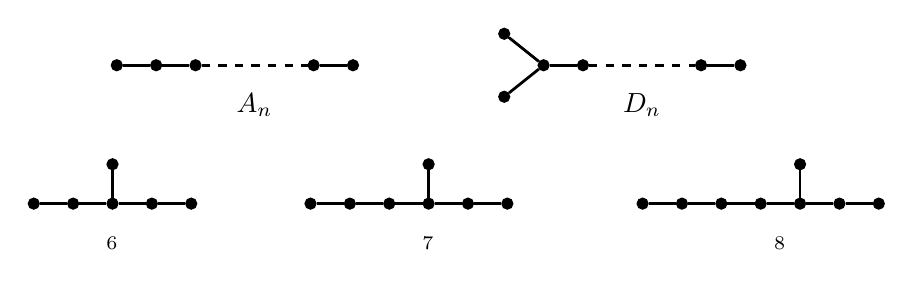
\begin{tikzpicture}
		\tikzset{dynode/.style={circle, draw, fill=black,
					minimum size=4pt, inner sep=0pt}}
		\tikzset{dyline/.style={line width=1pt}}
		\tikzset{dydash/.style={line width=1pt, dashed}}

		\begin{scope}[yshift=0, xshift=22em]
			\node[dynode] (a1) at (0,0) {};
			\node[dynode] (a2) at (0.5,0) {};
			\node[dynode] (a3) at (1,0) {};
			\node[dynode] (a4) at (1.5,0) {};
			\node[dynode] (a5) at (2,0) {};
			\node[dynode] (a6) at (2.5,0) {};
			\node[dynode] (a7) at (3,0) {};
			\node[dynode] (a8) at (2,0.5) {};

			\draw[dyline] (a1) -- (a2) -- (a3) -- (a4) -- (a5) -- (a6) -- (a7);
			\draw[dyline] (a5) -- (a8);

			\node[] (l) at (1.75,-0.5) {$\E_8$};
		\end{scope}

		\begin{scope}[yshift=0, xshift=10em]
			\node[dynode] (a1) at (0,0) {};
			\node[dynode] (a2) at (0.5,0) {};
			\node[dynode] (a3) at (1,0) {};
			\node[dynode] (a4) at (1.5,0) {};
			\node[dynode] (a5) at (2,0) {};
			\node[dynode] (a6) at (2.5,0) {};
			\node[dynode] (a8) at (1.5,0.5) {};

			\draw[dyline] (a1) -- (a2) -- (a3) -- (a4) -- (a5) -- (a6);
			\draw[dyline] (a4) -- (a8);

			\node[] (l) at (1.5,-0.5) {$\E_7$};
		\end{scope}

		\begin{scope}[yshift=0, xshift=0]
			\node[dynode] (a1) at (0,0) {};
			\node[dynode] (a2) at (0.5,0) {};
			\node[dynode] (a3) at (1,0) {};
			\node[dynode] (a4) at (1.5,0) {};
			\node[dynode] (a5) at (2,0) {};
			\node[dynode] (a8) at (1,0.5) {};

			\draw[dyline] (a1) -- (a2) -- (a3) -- (a4) -- (a5);
			\draw[dyline] (a3) -- (a8);

			\node[] (l) at (1,-0.5) {$\E_6$};
		\end{scope}

		\begin{scope}[yshift=5em, xshift=3em]
			\node[dynode] (a1) at (0,0) {};
			\node[dynode] (a3) at (0.5,0) {};
			\node[dynode] (a4) at (1,0) {};
			\node[dynode] (a5) at (2.5,0) {};
			\node[dynode] (a6) at (3.0,0) {};

			\draw[dyline] (a1) -- (a3) -- (a4);
			\draw[dydash] (a4) -- (a5);
			\draw[dyline] (a5) -- (a6);

			\node[] (l) at (1.75,-0.5) {$\op{A}_n$};
		\end{scope}

		\begin{scope}[yshift=5em, xshift=17em]
			\node[dynode] (a1) at (0,0.4) {};
			\node[dynode] (a2) at (0,-0.4) {};
			\node[dynode] (a3) at (0.5,0) {};
			\node[dynode] (a4) at (1,0) {};
			\node[dynode] (a5) at (2.5,0) {};
			\node[dynode] (a6) at (3.0,0) {};

			\draw[dyline] (a1) -- (a3);
			\draw[dyline] (a2) -- (a3);
			\draw[dyline] (a3) -- (a4);
			\draw[dydash] (a4) -- (a5);
			\draw[dyline] (a5) -- (a6);

			\node[] (l) at (1.75,-0.5) {$\op{D}_n$};
		\end{scope}
	\end{tikzpicture}
	\vspace{1em}
	\caption{\todo{describe}}
\end{figure}

Given a tree $T$ with weights $w$ in $\pi_{m-1}(\SO_m)$, we can form a manifold with boundary constructed in the following manner:
\begin{enumerate}
	\item For each vertex $v\in \op{Vert}(T)$, choose an $n$-disc bundle $\xi_v\to S^m_v$ classified by $w(v)\in \pi_{m-1}(\SO_m)$.
	\item For each edge $(v,w)\in \op{Edge}(T)$ connecting vertices $v$ and $w$, plumb together the bundles $\xi_v$ and $\xi_w$. For this to be well-defined, it's important to choose disjoint disc embeddings $\iota_{v,w} : D^m \to S^m_v$ for all $w$ connected to $v$.
	\item Smooth out the corners of the resulting space to get a manifold with boundary.
\end{enumerate}
\begin{definition}
	The \defn{plumbing} along the weighted tree $(T,w)$, denoted by $P(T,w)$ is the manifold with boundary described above.
\end{definition}

\begin{theorem}
	The result of this plumbing construction is independent of the choices of disc bundles $\xi_v$ and disc embeddings $\iota_{v,w} : D^m \to S^m_v$.
\end{theorem}

\begin{proof}
\end{proof}

\begin{remark}
	\todo{plumbing has a 1-skeleton homotopic to the tree}
\end{remark}

\begin{figure}[ht]
	\centering
	\import{graphics/temp-diagrams/}{spheres-connected-at-3-points.pdf_tex}
	\caption{A wedge of two spheres at $3$ points.}
\end{figure}

\begin{proposition}
	For each integer $q\geq 1$, there is a homotopy equivalence
	\[
		S^m\vee_q S^m \simeq S^m\vee S^m \vee \bigvee_{q-1} S^1,
	\]
	where $S^m\vee_q S^m$ denotes the wedge sum of two $m$-spheres at $q$ points.
\end{proposition}

\begin{proof}
\end{proof}

\subsection*{Plumbing Constructions of 3-Manifolds}
